\documentclass{article}
\usepackage{listings}
\usepackage{xcolor}
\usepackage{minted}
\usepackage{geometry}
\usepackage{booktabs}
\usepackage{float}
\usepackage{graphicx}

\geometry{
	textheight=9in,
	textwidth=6in,
	top=1in,
	headheight=12pt,
	headsep=25pt,
	footskip=30pt
}

\begin{document}
	
	\title{Artificial Intelligence Assignment 3}
	\author{12111620 Yixuan Ding}
	\date{\today}
	
	\maketitle
	
	\section*{Description}
	\subsection*{Brief Introduction}
	In this assignment, three main path-finding algorithms will be introduced and compared according to their time complexity and path length. The algorithms chosen are A*, Dijkstra and Bidirectional Breath-First Search. Further, difference heuristic function of A* algorithm will be consider, and their time complexity and path length will be compared, among which Manhattan distance, Euclidean distance will be considered as two measurement by viewing London Station in a flat plane, while great circle distance are measured based on the longitude and latitude of the point by considering the real situation in real world.
	
	\subsection*{Related Algorithm}
	\begin{itemize}
		\item \textbf{A*}\\
		A* is a path-finding algorithm which maintains priority queue of nodes to be explored and prioritize the node with lowest cost. The priority mechanism consider two parts: One is the sum of cost that taken to reach that node and the other is the heuristic estimate of the cost to reach the ultimate goal. The core idea of A* is estimating the cost needed to reach the goal, so choosing different heuristic function will influence the performance of the algorithm.
		\item \textbf{Dijkstra}\\
		Dijkstra complete path-finding job by maintains a set of nodes whose shortest distance from the source is known. In each iterations, the algorithm selects the node with the smallest known distance, explores its neighbors, and updates their distances if a shortest path is found.
		\item \textbf{Bidirectional Breath-First Search}\\
		In Bidirectional Breath-First Search, two BFS searches are performed concurrently: One starts from the source node and the other starts from the goal. Searches progress by exploring the neighbors layer by layer. The algorithm continues until a common node is found by both directions.
	\end{itemize}
	
	\subsection*{Related Heuristic Function}
	Heuristic functions below are all implemented only in A* algorithm. 
	\begin{itemize}
		\item \textbf{Manhattan Distance}
		Using Manhattan distance as the heuristic function in A* involves estimating the cost from the current node to the goal based on the horizontal and vertical distance in a grid-like environment:
		\begin{minted}[breaklines, breakafter=d]{python}
return abs(node_1_location[0] - node_2_location[0]) + abs(node_1_location[1] + node_2_location[1])
		\end{minted}
		\item \textbf{Euclidean Distance}
		The heuristic estimation based on euclidean distance involves employing the straight-line distance between the current node and the goal as an estimate for the remaining distance.
		 \begin{minted}[breaklines, breakafter=d]{python}
return math.sqrt((node_1_location[0] - node_2_location[0])**2 + (node_1_location[1] + node_2_location[1])**2)
		 \end{minted}
		\item \textbf{Great Circle Distance}
		The great-circle distance measures the shortest distance between two point on the Earth surface, considering the curvature of the planet. Such measurement guarantees the accuracy of the estimate.
		\begin{minted}[breaklines, breakafter=d]{python}
def geodistance(lng1,lat1,lng2,lat2):
lng1, lat1, lng2, lat2 = map(radians, [float(lng1), float(lat1), float(lng2), float(lat2)])
	dlon=lng2-lng1
	dlat=lat2-lat1
	a=sin(dlat/2)**2 + cos(lat1) * cos(lat2) * sin(dlon/2)**2
	distance=2*asin(sqrt(a))*6371*1000 
	distance=round(distance/1000,3)
	return distance
		\end{minted}
	\end{itemize}
	
	\section*{Result}
	\subsection*{Time Spent Comparison}
	\subsubsection*{Algorithm Aspect}
	Three algorithms introduced above are implemented and evaluated on \textbf{Every Path} between every two of London Stations. The overall spending time reflects the performance of each algorithm:
	\begin{table}[H]
		\centering
		\caption{Time Spent Comparison}
		\begin{tabular}{cc}
			\toprule
			Algorithm & Overall Time(s) \\
			\midrule
			A* &  17.0671 \\
			Dijkstra & 19.8989 \\
			Bidirectional-BFS & 15.3538  \\
			\bottomrule
		\end{tabular}
	\end{table}
	From the comparison, Bidirectional-BFS has best performance, and A* places second, while Dijkstra is the worst.
	
	\subsubsection*{Heuristic Function Aspect}
	Also, three heuristic functions are compared when implementing A* algorithm. The comparison are shown in the table:
	\begin{table}[H]
		\centering
		\caption{Time Spent Comparison}
		\begin{tabular}{cc}
			\toprule
			Heuristic Function & Overall Time(s) \\
			\midrule
			Manhattan &  15.1556 \\
			Euclidean & 16.7948 \\
			Great Circle &  28.0278 \\
			\bottomrule
		\end{tabular}
	\end{table}
	According to the table, using Manhattan distance as heuristic function have the shortest time. Time costs of implementing Manhattan and Euclidean distance 
	have relatively small difference, while using Great Circle as heuristic function spent much more time.
		
	\subsection*{Path Length Comparison}
	\subsubsection*{Algorithm Aspect}
	By going through the same path as before, the sum of length for each path is used for evaluating effectiveness of each algorithm, the shorter the overall length is, the better the algorithm is.
	\begin{table}[H]
		\centering
		\caption{Path Length Comparison}
		\begin{tabular}{cc}
			\toprule
			Algorithm & Overall Length(Degree) \\
			\midrule
			A* &  434022.8935 \\
			Dijkstra & 436746.3220 \\
			Bidirectional-BFS & 436950.1343 \\
			\bottomrule
		\end{tabular}
	\end{table}
	
	\subsubsection*{Heuristic Function Aspect}
	Now comes to evaluate the effectiveness of the choice of heuristic function of A* algorithm:
	\begin{table}[H]
		\centering
		\caption{Path Length Comparison}
		\begin{tabular}{cc}
			\toprule
			Heuristic Function & Overall Length(Degree) \\
			\midrule
			Manhattan &  435501.4628 \\
			Euclidean &  434022.8935 \\
			Great Circle &  432852.3090 \\
			\bottomrule
		\end{tabular}
	\end{table}
	
	\section*{Discussion}
	In the algorithm aspect, the running speed of A* is not slow, and A* has a shortest path length when finding path, making it a relatively useful algorithm. The reason why Bidirectional-BFS is so fast may due to the simplicity of the implementing scenario(the map is small and the search space is not that large). Potential guess is that A* algorithm may perform better when dealing with a large problem.\\
	As in the aspect of implementing heuristic function, Manhattan distance and Euclidean distance have similar running speed, which both outperforms Great Circle Distance. The reason of this is obvious: The calculation of the Great Circle is time-costing. However, the effectiveness of Great Circle Distance is also remarkable, the overall path length is a lot shorter than the other two algorithms. So when considering efficiency, choose Manhattan. While considering effectiveness, the Great Circle Distance is a better choice.
	
	\section*{Conclusion}
	In this assignment, three path-finding algorithms are selected to evaluate their performance on time spending task and path length task. Also, different heuristic function of A* algorithm are compared together. Overall, A* has a relatively good performance on those task, and may have better competitiveness when coming across a bigger problem. Every heuristic function has its own characteristic, and can be chosen according to different implementing needs.
	
	\section*{Appendix}
	\subsection*{Single Path Inference Example}
	Relatively short path: from \textit{White City} to \textit{Angel}
	\begin{figure}[H]
		\begin{minipage}{0.32\textwidth}
			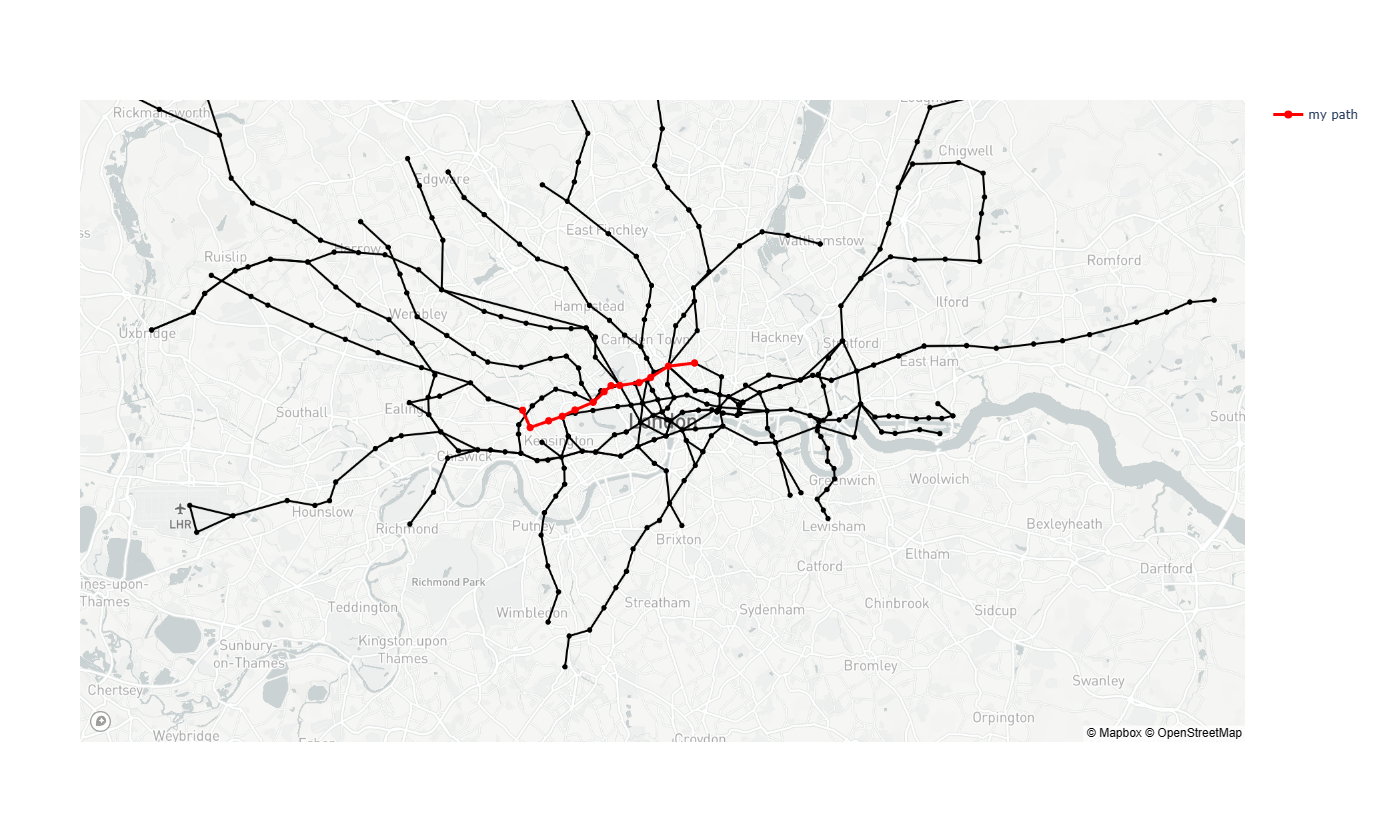
\includegraphics[width=\linewidth]{(short)_Astar.png}
			\caption{A*}
		\end{minipage}\hfill
		\begin{minipage}{0.32\textwidth}
			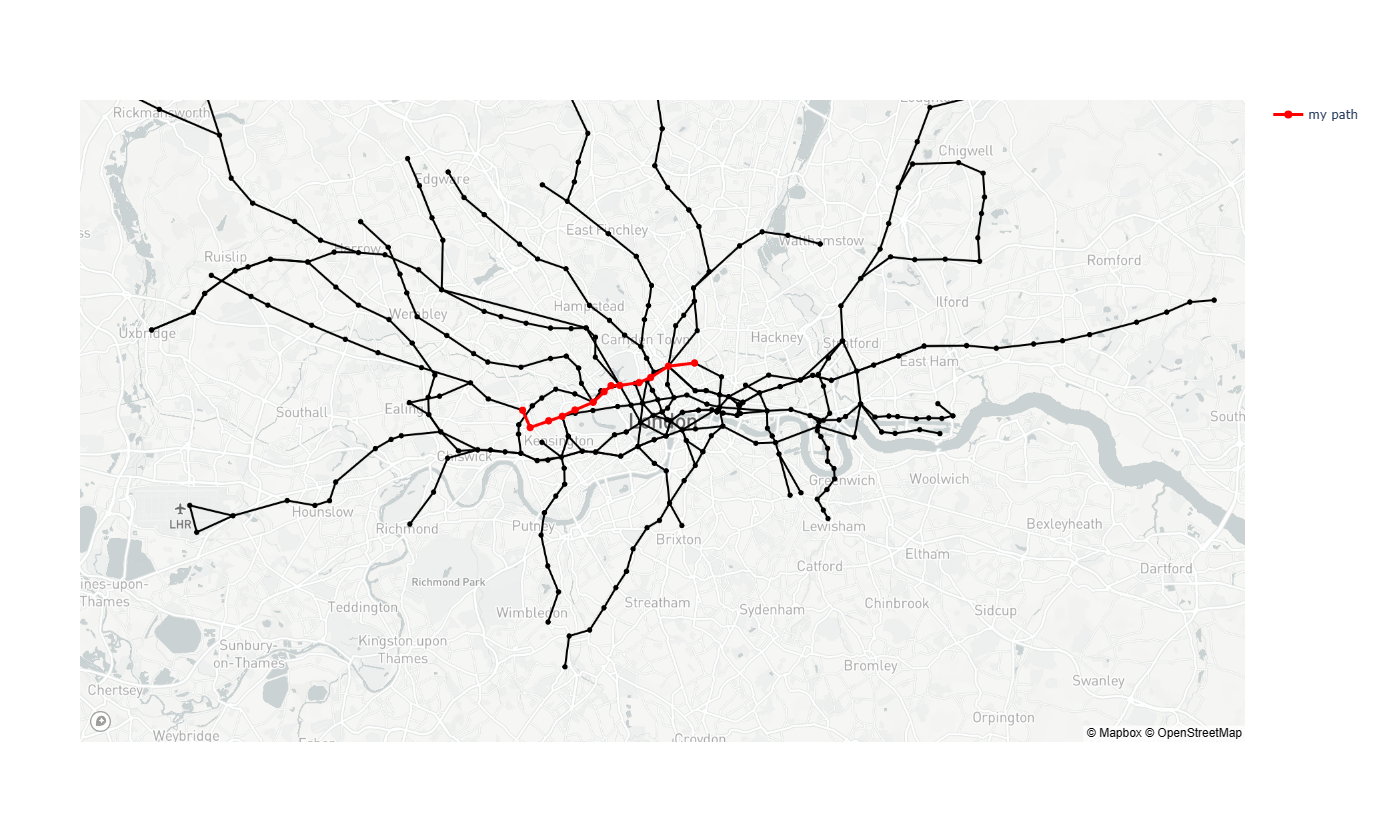
\includegraphics[width=\linewidth]{(short)_Dijkstra.png}
			\caption{Dijkstra}
		\end{minipage}\hfill
		\begin{minipage}{0.32\textwidth}
			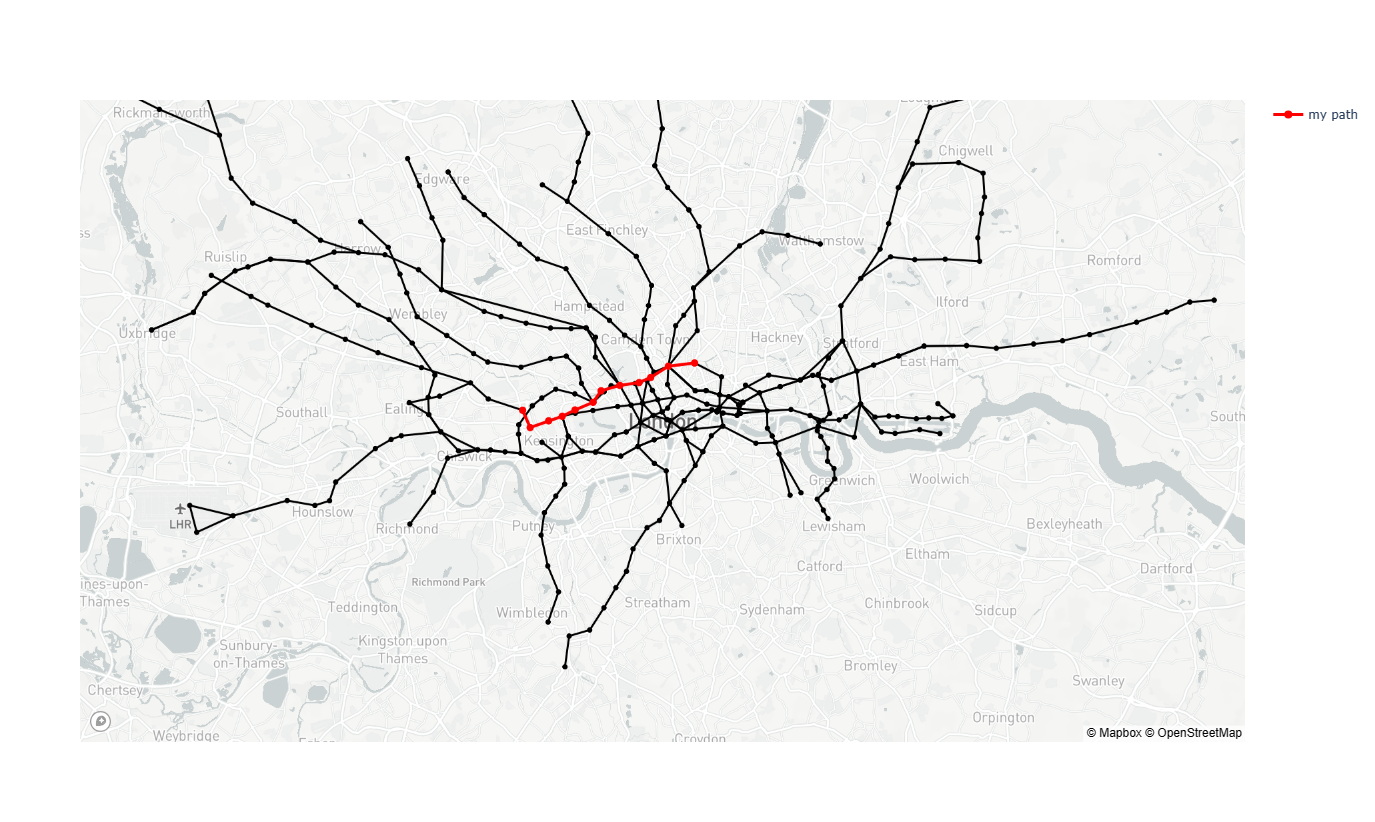
\includegraphics[width=\linewidth]{(short)_Bidirectional.png}
			\caption{Bidirectional}
		\end{minipage}
	\end{figure}
	
	Relatively long path: from \textit{Moor Park} to \textit{Beckton}
	\begin{figure}[H]
		\begin{minipage}{0.32\textwidth}
			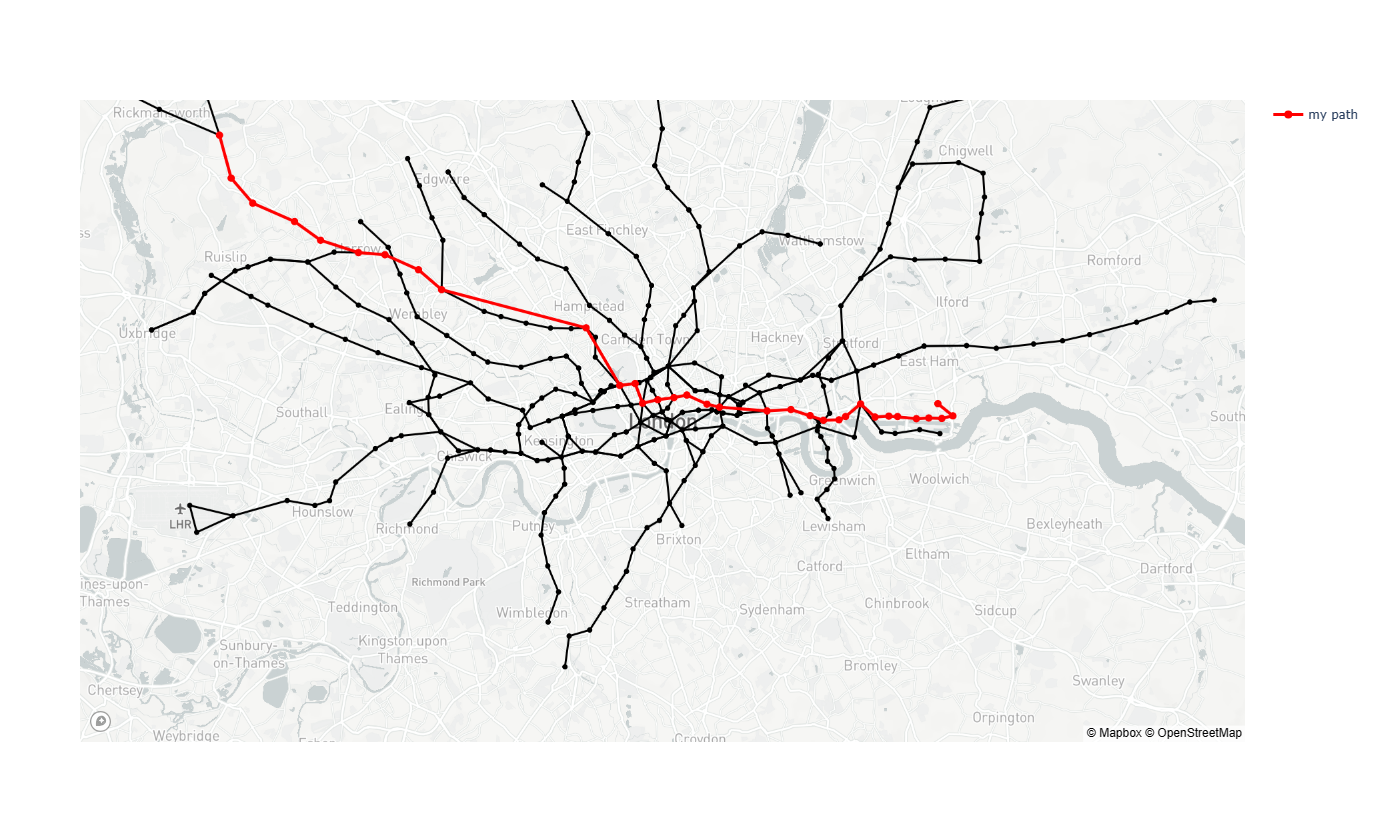
\includegraphics[width=\linewidth]{(long)_Astar.png}
			\caption{A*}
		\end{minipage}\hfill
		\begin{minipage}{0.32\textwidth}
			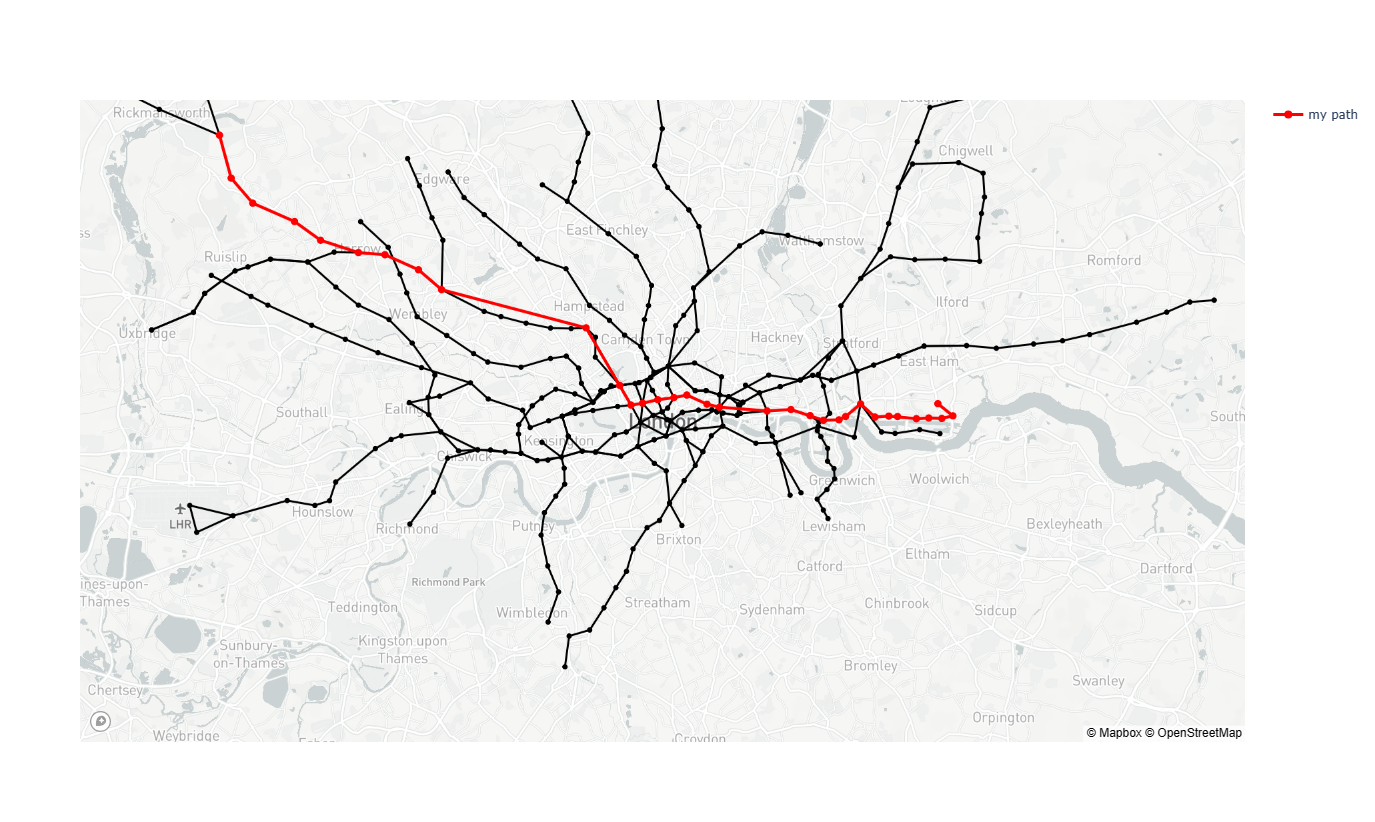
\includegraphics[width=\linewidth]{(long)_Dijkstra.png}
			\caption{Dijkstra}
		\end{minipage}\hfill
		\begin{minipage}{0.32\textwidth}
			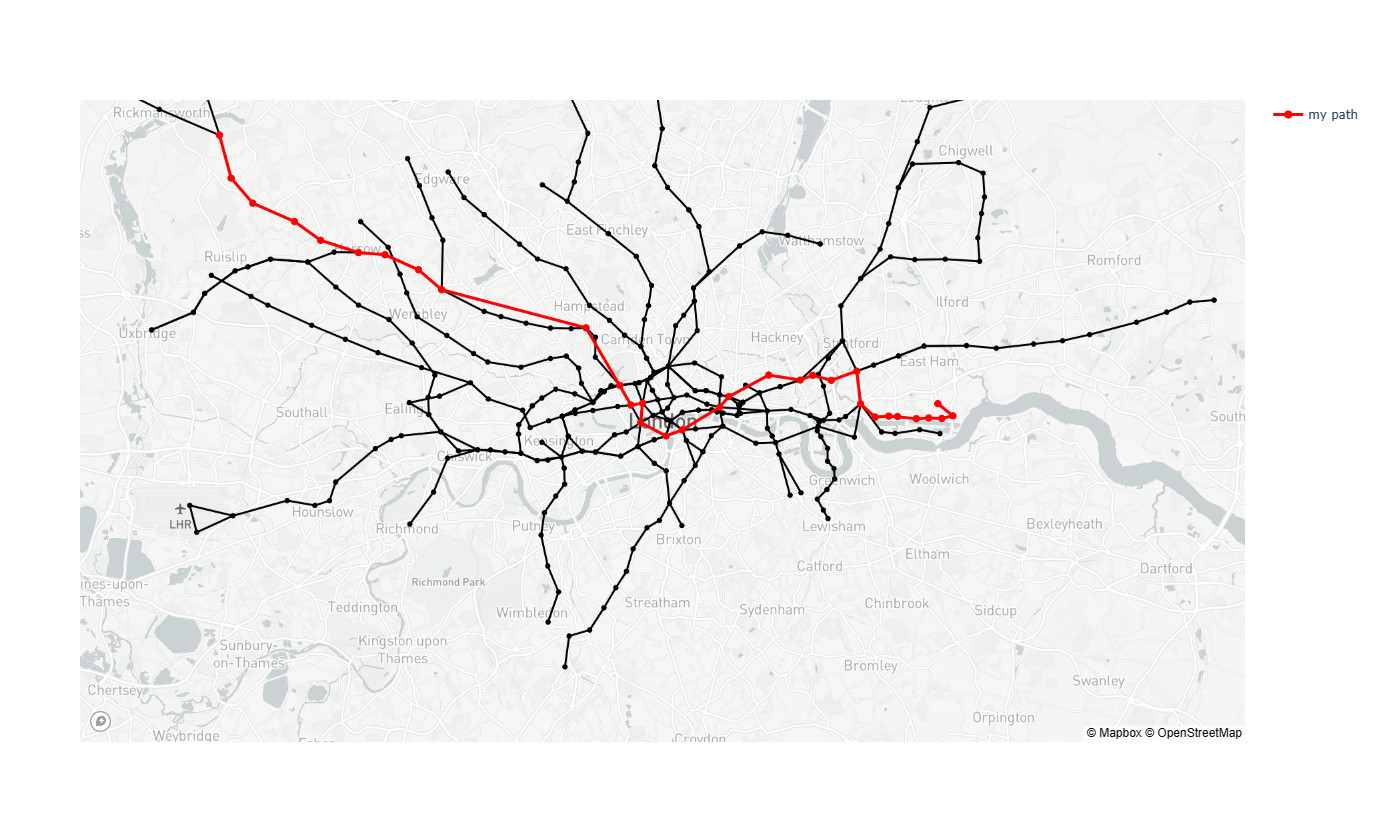
\includegraphics[width=\linewidth]{(long)_Bidirectional.png}
			\caption{Bidirectional}
		\end{minipage}
	\end{figure}
	%\nocite{1}
	 
	%\bibliographystyle{plain}
	%\bibliography{Reference.bib} 
\end{document}
